\section{Graphical Simulation}

As stated in the introduction, the goal of analysing the model proposed by Tanabe Kaneko\textsuperscript{\cite{tanabe1994behavior}} is to reduce the complexity of the equations of motion. The simpler model will reduce the number of actions required to calculate leaves positions and rotations. A scene is all objects and animations being rendered within a program. A simpler model would allow more objects and animations to be rendered which is desirable for more complex scenes.
\\
\\
\noindent The animation for the falling leaf was written from scratch in C++ using the OpenGL\textsuperscript{\textregistered} library. OpenGL\textsuperscript{\textregistered} is a library of functions and objects that allow developers to manipulate objects in a two dimensional or three dimensional vector space\textsuperscript{\cite{opengl}}. Doing this means that a physics engine can be made that purely maps the motion of a falling leaf.
\\
\\
\noindent Moving pictures are made up of individual frames changing at a rate such that the change in frames is indistinguishable. For the animation, the difference between two adjacent frames represents a discrete change in time, $\delta t$. This meant that the equations of motion are changed from functions to maps:

\begin{align}
\begin{split}
u_{n+1} &= u_{n} + \dot{u_{n}}\delta t, \\
v_{n+1} &= v_{n} + \dot{v_{n}}\delta t, \\
\omega_{n+1} &= \omega_{n} + \dot{\omega_{n}}\delta t, \\
x_{n+1} &= x_{n} + u_{n+1}\delta t, \\
y_{n+1} &= y_{n} + v_{n+1}\delta t, \\
\theta_{n+1} &= \theta_{n} + \omega_{n+1} \delta t,
\end{split}
\label{eq:discretetime}
\end{align}

\noindent where $n$ is the frame number, $u_{n}$, $v_{n}$, $\omega_{n}$, $x_{n}$, $y_{n}$ and $\theta_{n}$ are the horizontal velocity, vertical velocity, angular velocity, horizontal displacement, vertical displacement and angle respectively at frame $n$ and $\dot{u_{n}}$, $\dot{v_{n}}$ and $\dot{\omega_{n}}$ are the horizontal acceleration, vertical acceleration and angular acceleration respectively given by the Tanabe Kaneko equations of motion\textsuperscript{\cite{tanabe1994behavior}} using the values at frame $n$.
\\
\\
\noindent Equation~\ref{eq:discretetime} is then implemented into a physics engine that will update the new positions and rotations of each card at each frame. The vertical position is allocated to the $y$ axis and the horizontal position in the $x$ axis meaning there is no $z$ axis motion implemented. These values will then be taken, turned into transformations and applied to each leaf when the frame is updated. These frames are then played one after another with a maximum value of 60 frames per second (fps). Before testing how many leaves it is possible to render before a visible effect on the fps takes place, it is necessary to make sure the equations are being used and are correctly calculating position and angle. This is checked by having a single leaf fall. Producing different shapes using triangles is called tessellation. The leaf in the simulation is a purple square tessellated with two triangles. This reduces the time taken to render the shape as little as possible whilst looking like a piece of paper falling.

\begin{figure}[H]
\centering
	\begin{subfigure}[b]{0.4\textwidth}
		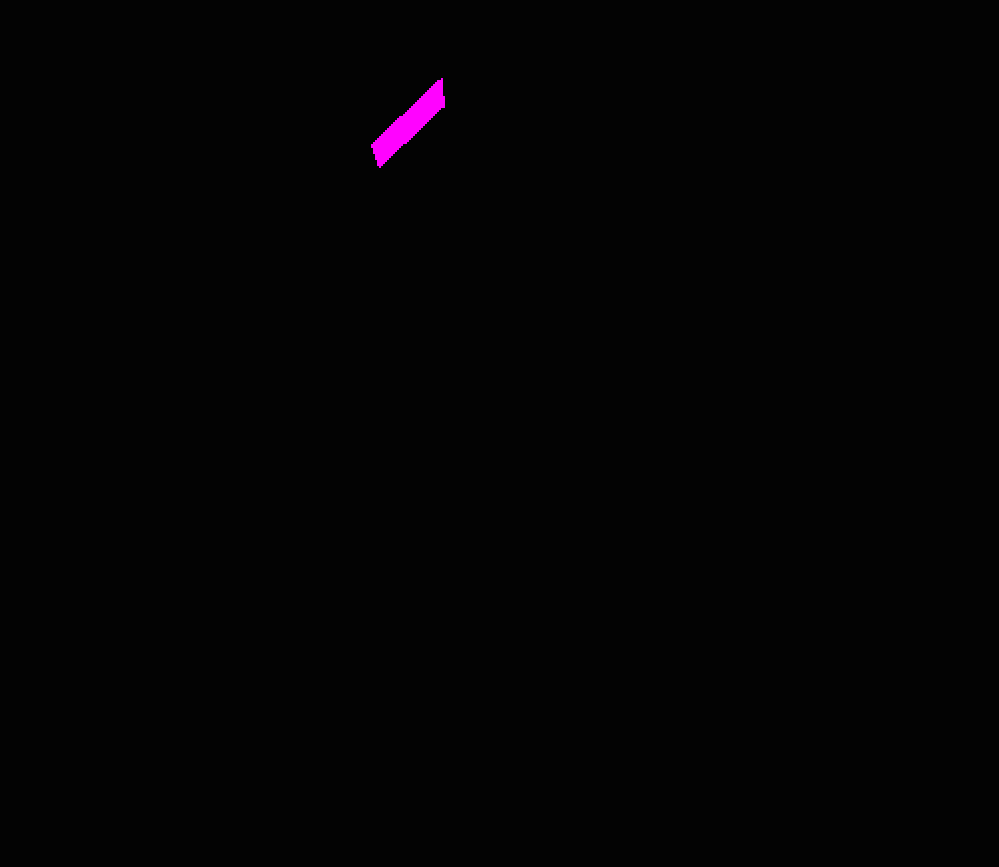
\includegraphics[width=\textwidth]{Motion_Graphs/single_leaf.png}
    	\caption{\label{fig:singlefloat}}
    \end{subfigure}
    \begin{subfigure}[b]{0.395\textwidth}
		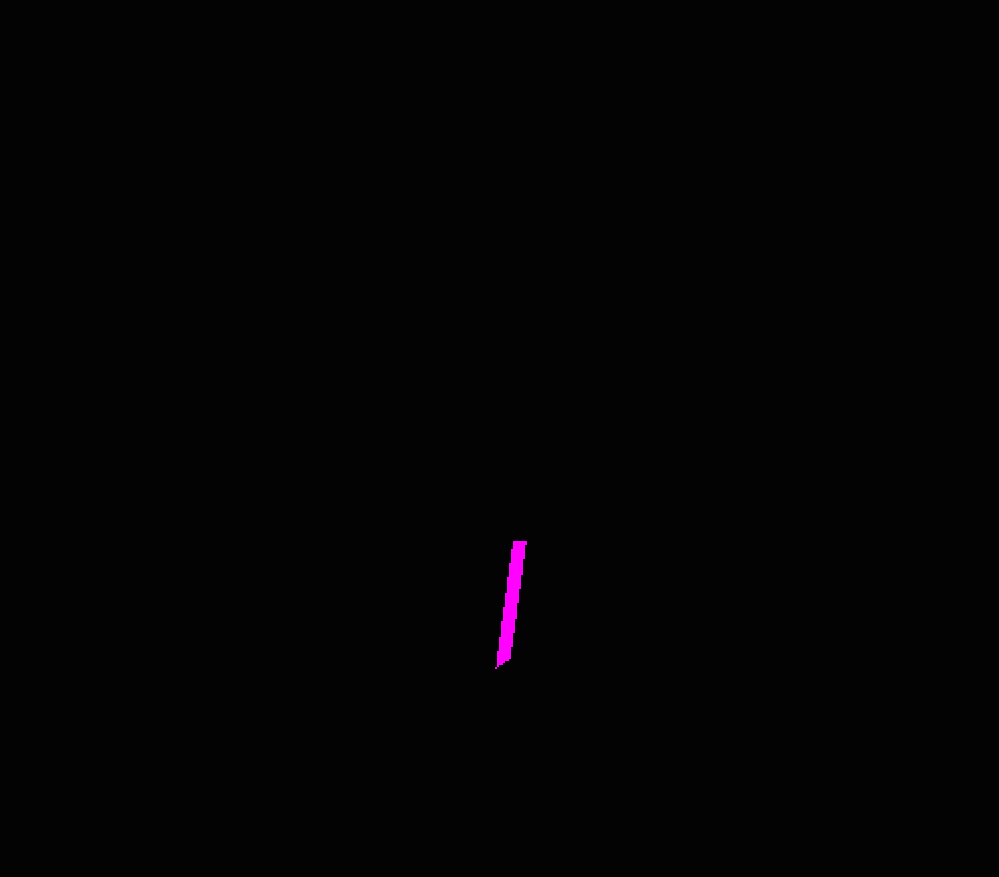
\includegraphics[width=\textwidth]{Motion_Graphs/single_equil.png}
    	\caption{\label{fig:singlefall}}
    \end{subfigure}
\caption{\label{fig:fallingleaf}The simulation with one square. (Left) The square falls as expected from real world and simulation data. (Right) The square reaches a limit cycle with very small deviation which makes it appear to be falling on its side.}
\end{figure}

\noindent For a duration of the fall, the square exhibits behavior seen in real world testing and the simulation produced in Section~\ref{sec:motion}. After the angle of the square becomes $\pm\frac{\pi}{2}$, the square oscillates around $\frac{\pi}{2}$ with such a small deviation it seems to fall straight, as can be seen in Figure~\ref{fig:singlefall}. More squares can still be added and the fps measured for increased number of falling squares.

\begin{figure}[H]
\centering
	\begin{subfigure}[b]{0.3\textwidth}
		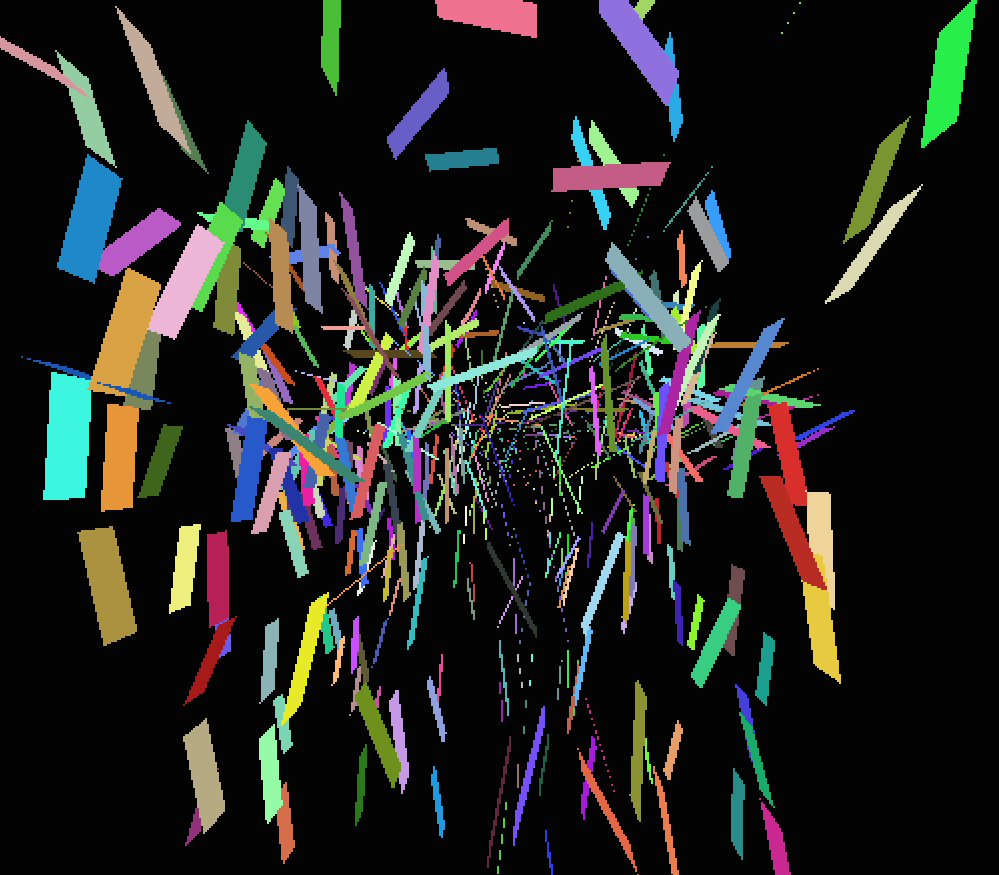
\includegraphics[width=\textwidth]{Motion_Graphs/500_leaves.png}
    	\caption{\label{fig:500leaves}500 squares.}
    \end{subfigure}
    \begin{subfigure}[b]{0.3\textwidth}
		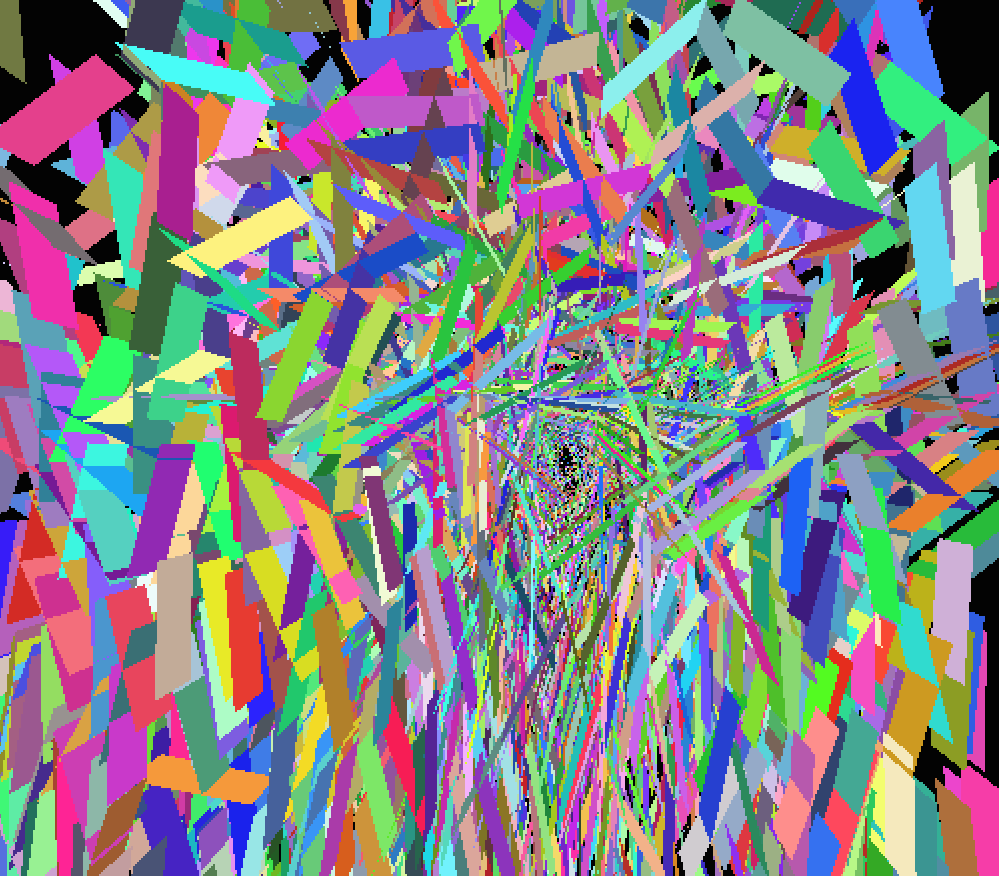
\includegraphics[width=\textwidth]{Motion_Graphs/13000_leaves.png}
    	\caption{\label{fig:13000leaves}13000 squares.}
    \end{subfigure}
    \begin{subfigure}[b]{0.3\textwidth}
		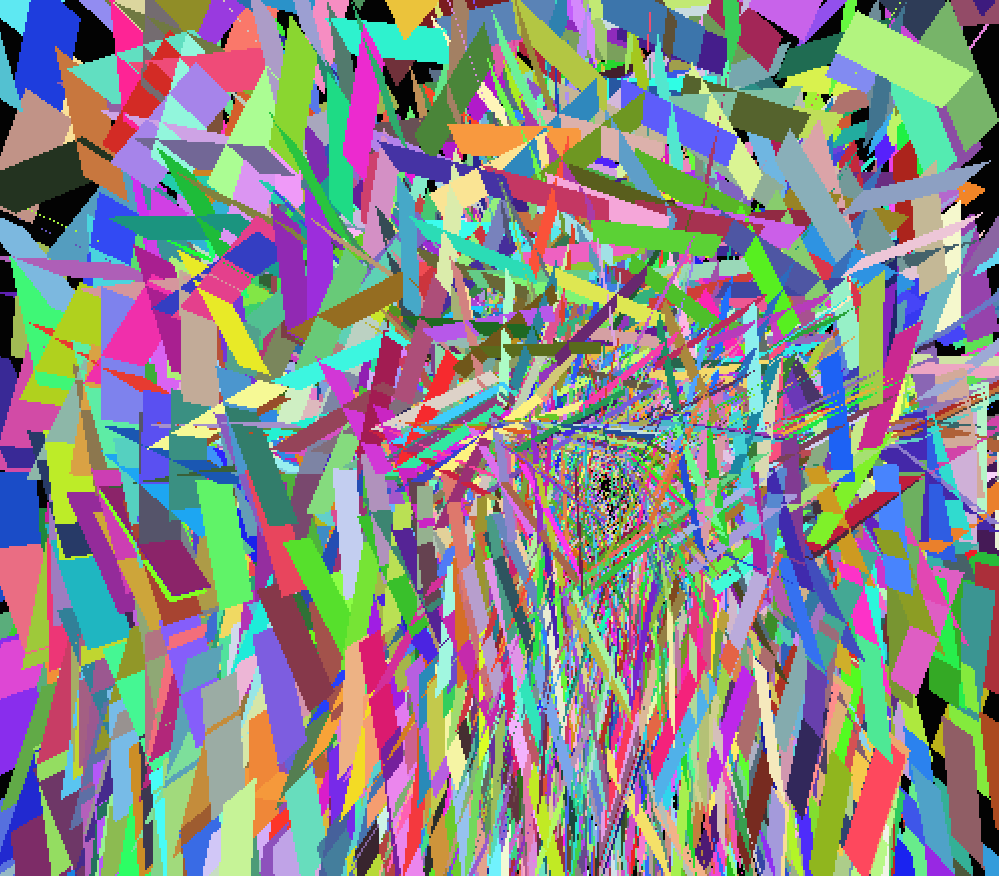
\includegraphics[width=\textwidth]{Motion_Graphs/15000_leaves.png}
    	\caption{\label{fig:15000leaves}15000 squares.}
    \end{subfigure}
\caption{\label{fig:fallingleaves}The simulation with 500 (Left), 13000 (Middle) and 15000 (Right) squares falling. All are given random initial conditions of $x$ position between $(-10,10)$, $y$ position of $(10)$ $z$ position between $(-65,-15)$ and angle between $(-\frac{\pi}{2},\frac{\pi}{2})$ relative to the origin of the space. The camera is placed at coordinates $(0,1,0).$}
\end{figure}

\noindent In Figure~\ref{fig:fallingleaves}, there are three examples of the simulation running with multiple falling leaves. The colour of the squares have been chosen to be random such that it is possible to distinguish between different squares. Figure~\ref{fig:500leaves} shows the simulation running with 500 squares. It runs at approximately 60 fps with little to no deviation from 60. The frame rate does not change until 13000 squares are rendered (Figure~\ref{fig:13000leaves}). At this point the frame rate deviates by a small amount around 59 fps. From there, the frame rate decreases as you increase the number of squares in a linear fashion. Jumps between frames become very visible as you reach 15000 squares (Figure~\ref{fig:15000leaves}). It can also be noted a vast majority of the squares have an angle of approximately $\frac{\pi}{2}$ in Figure~\ref{fig:fallingleaves} because the angles of the square reach a limit cycle based closely around that value.
\\
\\
Having 13000 falling pieces of paper on screen may seem like a lot, but this animation uses simple squares made only using two triangles. In animation made to look realistic, leaves and papers will be rendered using hundreds of triangles. The correlation between tessellation and memory usage may not be linear but it is probable that the animation could not handle as many fully rendered leaves or papers. 